% AA-56
\chapter{Macierze Cartana, układy korzeni i grupy Weyla}
\label{aa:ch:root-systems}

Grafy McKaya z rozdziału~\ref{aa:ch:mckay} prowadzą do
macierzy $2I-A$. W tym rozdziale zbadamy również macierze
dodatnio określone oraz wyjaśnimy ich związek z geometrią
skończonych układów korzeni. Będziemy pracować w rzeczywistych
przestrzeniach euklidesowych skończonego wymiaru.

\section{Macierze Cartana i grafy McKaya}

\begin{definicja}[Uogólniona macierz Cartana]
\label{aa:def:generalized-cartan}
Uogólnioną macierzą Cartana stopnia $n\ge1$ nazywamy
macierz całkowitą $C=(c_{ij})_{i,j=1}^n$ taką, że
$c_{ii}=2$, dla $i\ne j$ mamy $c_{ij}\le0$, a
$c_{ij}=0$ wtedy i tylko wtedy, gdy $c_{ji}=0$.
Macierz jest symetryzowalna, jeżeli istnieje dodatnia
macierz diagonalna $D$ taka, że $DC$ jest symetryczna.
Mówimy, że jest typu skończonego, jeśli jest
symetryzowalna i $DC$ jest dodatnio określona.
W grafie macierzy łączymy różne wierzchołki $i,j$,
jeżeli $c_{ij}\ne0$. Nierozkładalność oznacza
spójność tego grafu.
\end{definicja}

\begin{stwierdzenie}[Postać kwadratowa macierzy McKaya]
\label{aa:prop:mckay-cartan}
Niech $G$ będzie niecykliczną skończoną podgrupą
$\operatorname{SL}_2(\mathbb C)$ albo nietrywialną grupą
cykliczną w tej grupie. Niech $A$ będzie jej macierzą
McKaya, a $d$ kolumną wymiarów reprezentacji
nieprzywiedlnych. Wówczas $C=2I-A$ jest symetryczną
uogólnioną macierzą Cartana, dodatnio półokreśloną,
z jądrem $\mathbb R d$. Usunięcie dowolnego wiersza
i odpowiadającej mu kolumny daje macierz dodatnio określoną.
\end{stwierdzenie}
\begin{proof}
Z Twierdzeń~\ref{aa:tw:mckay-properties}
i~\ref{aa:tw:mckay-ade} oraz
Przykładu~\ref{aa:prz:mckay-cyclic} wiemy, że $A$
jest symetryczna, ma zera na przekątnej, jej graf jest
spójny oraz $Ad=2d$, gdzie $d_i>0$.
Dla $x\in\mathbb R^n$ mamy
\[
\begin{aligned}
 \sum_{i<j}a_{ij}d_id_j
  \left(\frac{x_i}{d_i}-\frac{x_j}{d_j}\right)^2
 &=\sum_i \frac{x_i^2}{d_i}\sum_j a_{ij}d_j
       -2\sum_{i<j}a_{ij}x_ix_j\\
 &=2\sum_i x_i^2-\sum_{i,j}a_{ij}x_ix_j
 =x^{\mathsf T}Cx.
\end{aligned}
\]
Suma jest nieujemna i znika dokładnie wtedy, gdy
$x_i/d_i=x_j/d_j$ na każdej krawędzi. Spójność
oznacza, że wszystkie te ilorazy są równe. Ponieważ
$Cd=0$, otrzymujemy dokładnie wskazane jądro.
Dla macierzy głównej po usunięciu indeksu $i$ rozważamy
wektory $x$ o współrzędnej $x_i=0$. Jeżeli taki
wektor ma zerową formę kwadratową, to $x=td$,
a $0=td_i$ daje $t=0$. Forma ograniczona jest więc
dodatnio określona.
\end{proof}

Grupa trywialna ma macierz McKaya $(2)$, zatem
$2I-A=(0)$ nie spełnia definicji uogólnionej macierzy
Cartana. Jest to osobny przypadek brzegowy.

\section{Skończone układy korzeni}

\begin{definicja}[Zredukowany krystalograficzny układ korzeni]
\label{aa:def:root-system}
Niech $E$ będzie rzeczywistą przestrzenią euklidesową
dodatniego wymiaru. Skończony zbiór $\Phi\subset E\setminus\{0\}$
nazywamy zredukowanym krystalograficznym układem korzeni,
jeżeli:
\begin{enumerate}
\item $\operatorname{span}_{\mathbb R}\Phi=E$;
\item $\Phi\cap\mathbb R\alpha=\{\alpha,-\alpha\}$
      dla każdego $\alpha\in\Phi$;
\item odbicie $s_\alpha(x)=x-
      \frac{2(x,\alpha)}{(\alpha,\alpha)}\alpha$
      spełnia $s_\alpha(\Phi)=\Phi$ dla każdego $\alpha\in\Phi$;
\item $\frac{2(\beta,\alpha)}{(\alpha,\alpha)}\in\mathbb Z$
      dla wszystkich $\alpha,\beta\in\Phi$.
\end{enumerate}
Grupa Weyla $W(\Phi)$ jest podgrupą grupy ortogonalnej
generowaną przez wszystkie $s_\alpha$ dla $\alpha\in\Phi$.
Układ jest nierozkładalny, jeśli nie można rozdzielić
$\Phi$ na dwa niepuste wzajemnie ortogonalne podzbiory.
\end{definicja}

\begin{lemat}[Różnica korzeni]
\label{aa:lem:root-difference}
Niech $\alpha,\beta$ będą różnymi, nieproporcjonalnymi
korzeniami układu $\Phi$ z Definicji~\ref{aa:def:root-system}.
Jeśli $(\alpha,\beta)>0$, to $\alpha-\beta\in\Phi$.
\end{lemat}
\begin{proof}
Liczby $p=2(\alpha,\beta)/(\alpha,\alpha)$ oraz
$q=2(\alpha,\beta)/(\beta,\beta)$ są dodatnimi
liczbami całkowitymi. Ze ścisłej nierówności
Cauchy'ego--Schwarza dla nieproporcjonalnych wektorów
wynika $pq=4(\alpha,\beta)^2/
((\alpha,\alpha)(\beta,\beta))<4$.
Co najmniej jedna z liczb $p,q$ jest równa $1$.
Jeśli $q=1$, to $s_\beta(\alpha)=\alpha-\beta\in\Phi$.
Jeśli $p=1$, to $s_\alpha(\beta)=\beta-\alpha\in\Phi$,
więc także jej przeciwieństwo należy do $\Phi$.
\end{proof}

\begin{definicja}[Baza i korzenie dodatnie]
\label{aa:def:root-base}
Niech $\Phi$ będzie zredukowanym krystalograficznym
układem korzeni w $E$. Bazą układu nazywamy bazę
$\Delta=(\alpha_1,\ldots,\alpha_n)$ przestrzeni $E$
złożoną z korzeni, względem której współrzędne
każdego korzenia są całkowite i albo wszystkie
nieujemne, albo wszystkie niedodatnie.
Korzenie z pierwszej klasy nazywamy dodatnimi,
z drugiej ujemnymi; zbiory te oznaczamy
$\Phi^+$ oraz $\Phi^-$.
Elementy $\Delta$ nazywamy korzeniami prostymi.
\end{definicja}

\begin{twierdzenie}[Istnienie bazy układu]
\label{aa:tw:root-base}
Niech $\Phi$ będzie układem jak w
Definicji~\ref{aa:def:root-system}. Dla każdego
$h\in E$ takiego, że $(h,\alpha)\ne0$ dla
wszystkich $\alpha\in\Phi$, istnieje baza układu,
dla której $\Phi^+=\{\alpha\in\Phi:(h,\alpha)>0\}$.
Różne elementy tej bazy mają niedodatni iloczyn skalarny.
\end{twierdzenie}
\begin{proof}
Taki wektor $h$ istnieje, ponieważ skończona suma
właściwych hiperpłaszczyzn nie może pokryć $E$
(na przykład iloczyn ich niezerowych równań liniowych
jest niezerowym wielomianem).
W zbiorze korzeni o $(h,\alpha)>0$ wybierzmy wszystkie
korzenie nierozkładalne na sumę dwóch korzeni z tego
samego zbioru; niech $\Delta$ będzie ich zbiorem.
Każdy dodatni korzeń jest sumą elementów $\Delta$:
uporządkujmy skończony zbiór dodatnich wartości
$(h,\alpha)$ rosnąco. Jeżeli korzeń nie należy do
$\Delta$, to $\alpha=\beta+\gamma$, gdzie
$(h,\beta),(h,\gamma)>0$ są obie mniejsze od
$(h,\alpha)$. Indukcja po tym uporządkowaniu
daje rozkład obu składników, a więc i $\alpha$.
Każdy ujemny korzeń jest przeciwieństwem dodatniego.

Dla różnych $\alpha,\beta\in\Delta$ nie mogą one być
proporcjonalne, ponieważ układ jest zredukowany,
a oba korzenie dodatnie. Gdyby $(\alpha,\beta)>0$,
Lemat~\ref{aa:lem:root-difference} dałby korzeń
$\alpha-\beta$. Jeśli jest dodatni, rozkład
$\alpha=(\alpha-\beta)+\beta$ przeczy wyborowi $\alpha$.
Jeśli jest ujemny, rozkład
$\beta=(\beta-\alpha)+\alpha$ przeczy wyborowi $\beta$.
Zatem $(\alpha,\beta)\le0$.

Aby dowieść niezależności liniowej $\Delta$, rozważmy
równość $\sum_{\alpha\in\Delta}t_\alpha\alpha=0$.
Rozdzielmy dodatnie i ujemne współczynniki:
$u=\sum_{t_\alpha>0}t_\alpha\alpha
=\sum_{t_\beta<0}(-t_\beta)\beta=v$.
Z niedodatnich iloczynów skalarnych między rozłącznymi
rodzinami wynika $(u,v)\le0$. Ponieważ $u=v$,
mamy $\|u\|^2\le0$, więc $u=v=0$. Każdy niepusty
z tych dwóch dodatnich składników miałby dodatni
iloczyn skalarny z $h$, sprzeczność.
Wszystkie współczynniki są więc zerowe.
Z wcześniejszego rozkładu korzeni oraz faktu,
że $\Phi$ rozpina $E$, wynika, że $\Delta$ rozpina $E$.
Rozkłady są zatem całkowitymi współrzędnymi
w bazie, o wymaganych znakach.
\end{proof}

\begin{twierdzenie}[Odbicia proste i komory Weyla]
\label{aa:tw:weyl-chambers}
Niech $\Delta=(\alpha_1,\ldots,\alpha_n)$ będzie
bazą skończonego układu korzeni $\Phi$ w $E$.
Wówczas każdy korzeń jest obrazem pewnego korzenia
prostego przez iloczyn odbić prostych $s_{\alpha_i}$.
Grupa $W(\Phi)$ jest skończona i generowana przez te
odbicia. Dowolne dwie bazy układu jako zbiory są
przeprowadzane jedna na drugą przez element $W(\Phi)$.
Grupa działa przechodnio na składowych spójności
zbioru $E\setminus\bigcup_{\alpha\in\Phi}\alpha^\perp$,
zwanych komorami Weyla. Jedna z komór ma postać
$\mathcal C=\{x\in E:(x,\alpha_i)>0,\ i=1,\ldots,n\}$.
\end{twierdzenie}
\begin{proof}
Grupa Weyla permutuje skończony zbiór $\Phi$.
Jeśli element grupy ustala każdy korzeń, ustala ich
rozpiętość $E$, czyli jest identycznością. Działanie
jest wierne, zatem grupa jest skończona.

Dla dodatniego korzenia $\beta=\sum_i k_i\alpha_i$
definiujemy wysokość $\sum_i k_i$. Jeśli $\beta$
nie jest prosty, to z
$(\beta,\beta)=\sum_i k_i(\alpha_i,\beta)>0$
wynika istnienie $i$ z $k_i>0$ i
$(\alpha_i,\beta)>0$. Wtedy
$s_{\alpha_i}(\beta)=\beta-m\alpha_i$ dla dodatniej
liczby całkowitej $m$ i jest korzeniem.
Gdyby $\beta$ miał tylko jedną niezerową współrzędną,
byłby dodatnią wielokrotnością $\alpha_i$, a z redukcji
wynikałoby $\beta=\alpha_i$, wbrew założeniu.
Zatem co najmniej jedna współrzędna poza $i$
jest dodatnia i nie zmienia się w odbiciu.
Wszystkie współrzędne odbitego korzenia są wobec tego
nieujemne (nie mogą być wszystkie niedodatnie).
Jego wysokość zmalała o $m>0$.
Indukcja kończy się na korzeniu prostym.
Dla korzenia ujemnego stosujemy argument do jego
przeciwieństwa i korzystamy z $-\alpha_i=s_{\alpha_i}(\alpha_i)$.
Dla izometrii $w$ zachodzi $s_{w\alpha}=ws_\alpha w^{-1}$,
co widać przez podstawienie do wzoru na odbicie.
Każde odbicie korzeniowe należy więc do podgrupy
generowanej przez odbicia proste.

Zbiór $\mathcal C$ jest niepusty, gdyż istnieje
wektor $h$ określony równaniami $(h,\alpha_i)=1$
(baza gwarantuje jednoznaczną rozwiązywalność).
Jest wypukły, a dla każdego korzenia znak iloczynu
z $x\in\mathcal C$ jest ustalony przez znak jego
współrzędnych. Z drugiej strony znak $(x,\alpha_i)$
nie może się zmienić w żadnej składowej spójności
dopełnienia hiperpłaszczyzn. Zatem $\mathcal C$
jest dokładnie jedną składową.
Weźmy dowolny $x$ w tym dopełnieniu. Skończoność grupy
daje element $w$, dla którego $(wx,h)$ jest maksymalne
w orbicie. Jeśli $(wx,\alpha_i)<0$, to
\[
 (s_{\alpha_i}wx,h)-(wx,h)
 =-\frac{2(wx,\alpha_i)(\alpha_i,h)}{(\alpha_i,\alpha_i)}>0,
\]
co przeczy maksymalności. Równość zera jest niemożliwa,
bo grupa permutuje hiperpłaszczyzny korzeniowe.
Stąd $wx\in\mathcal C$. Ponieważ izometrie grupy
przeprowadzają składowe dopełnienia na składowe,
działanie na komorach jest przechodnie.

Niech $\Delta'$ będzie inną bazą, a $\mathcal C'$
jej komorą zdefiniowaną analogicznie. Istnieje
$w\in W(\Phi)$ takie, że $w\mathcal C=\mathcal C'$.
Jeżeli $x\in\mathcal C$, to
$(wx,w\beta)=(x,\beta)$ dla każdego $\beta\in\Phi$.
Zatem $w$ przeprowadza dodatnie korzenie względem
$\Delta$ na dodatnie korzenie względem $\Delta'$.
W dowolnej bazie korzeń prosty nie jest sumą dwóch
dodatnich korzeni, ponieważ jego współrzędne
tworzą wektor jednostkowy. Odwrotnie, dowód
Twierdzenia~\ref{aa:tw:root-base} pokazuje, że wszystkie
nierozkładalne dodatnie korzenie tworzą bazę.
Ponieważ zawierają już wszystkie elementy danej
bazy, nie mogą zawierać żadnych dodatkowych elementów.
Liniowość i odwracalność $w$ zachowują nierozkładalność
na sumę dodatnich korzeni, więc $w\Delta=\Delta'$.
\end{proof}

\section{Macierz układu i diagram Dynkina}

\begin{twierdzenie}[Macierz Cartana układu korzeni]
\label{aa:tw:root-cartan}
Niech $\Phi$ będzie skończonym układem korzeni jak wyżej,
a $\Delta=(\alpha_i)_{i=1}^n$ jego bazą.
Macierz
\[
 c_{ij}=\frac{2(\alpha_i,\alpha_j)}{(\alpha_i,\alpha_i)}
\]
jest uogólnioną macierzą Cartana typu skończonego.
Jeżeli $i\ne j$, to $c_{ij}c_{ji}\in\{0,1,2,3\}$.
Ponadto układ jest nierozkładalny wtedy i tylko wtedy,
gdy graf macierzy jest spójny.
\end{twierdzenie}
\begin{proof}
Dla dowolnej bazy układu w sensie
Definicji~\ref{aa:def:root-base} wektor określony przez
$(h,\alpha_i)=1$ wyznacza dokładnie te same korzenie
dodatnie. Korzenie proste są nierozkładalne na dwa
dodatnie: ich współrzędne są wektorami jednostkowymi.
Każdy inny dodatni korzeń nie może być nierozkładalny,
gdyż dowód Twierdzenia~\ref{aa:tw:root-base} tworzy
bazę z nierozkładalnych, a ta zawiera już wszystkie
$\alpha_i$. Zatem również dla tej bazy różne
korzenie proste mają niedodatnie iloczyny skalarne.
Całkowitość wynika z aksjomatu krystalograficzności.
Dla $D=\operatorname{diag}((\alpha_i,\alpha_i)/2)$
macierz $DC$ jest macierzą Grama bazy, a więc jest
symetryczna i dodatnio określona:
$x^{\mathsf T}DCx=\|\sum_i x_i\alpha_i\|^2>0$
dla $x\ne0$.
Dla różnych $i,j$ ścisła nierówność Cauchy'ego--Schwarza
daje $0\le c_{ij}c_{ji}<4$, co daje listę.

Jeżeli graf jest niespójny, przestrzenie rozpięte
przez korzenie proste z poszczególnych składowych
są wzajemnie ortogonalne. Odbicia proste zachowują
każdą z tych przestrzeni i działają identycznościowo
na pozostałych. Z Twierdzenia~\ref{aa:tw:weyl-chambers}
każdy korzeń jest w orbicie korzenia prostego,
więc należy do jednej z tych przestrzeni.
Otrzymujemy rozkład ortogonalny układu.
Jeśli zaś $\Phi=\Phi_1\sqcup\Phi_2$ jest rozkładem
na dwa niepuste ortogonalne podzbiory, oba zawierają
korzenie proste: w przeciwnym razie jeden z nich
byłby ortogonalny do całej bazy, niemożliwe dla
niezerowego korzenia. Pomiędzy tymi częściami
nie ma krawędzi.
\end{proof}

\begin{definicja}[Diagram Dynkina]
\label{aa:def:dynkin}
Dla macierzy Cartana typu skończonego rysujemy między
$i,j$ krawędź o krotności $c_{ij}c_{ji}$, jeśli
iloczyn jest niezerowy. Przy krawędzi wielokrotnej
strzałka wskazuje koniec odpowiadający krótszemu
korzeniowi. W konwencji z Twierdzenia~\ref{aa:tw:root-cartan}
oznacza to wierzchołek $i$ wtedy, gdy
$|c_{ij}|>|c_{ji}|$. W przypadku abstrakcyjnej
macierzy symetryzowalnej porównujemy dodatnie
wpisy symetryzatora $D$, odpowiadające połowom
kwadratów długości korzeni.
\end{definicja}

\section{Klasyfikacja macierzy typu skończonego}

\begin{twierdzenie}[Klasyfikacja diagramów skończonych]
\label{aa:tw:finite-dynkin}
Każda nierozkładalna uogólniona macierz Cartana typu
skończonego ma, z dokładnością do jednoczesnej
permutacji wierszy i kolumn, jeden z diagramów
$A_n$ ($n\ge1$), $B_n,C_n$ ($n\ge2$),
$D_n$ ($n\ge4$), $E_6,E_7,E_8,F_4,G_2$.
Tutaj $B_2$ i $C_2$ są równoważne po zamianie wierzchołków.
Wszystkie wymienione macierze są typu skończonego.
\end{twierdzenie}
\begin{proof}
Niech $D$ będzie dodatnim symetryzatorem.
Macierz $S=D^{1/2}CD^{-1/2}$ jest symetryczna
i dodatnio określona, bo jest równa
$D^{-1/2}(DC)D^{-1/2}$. Ma przekątną $2$,
a jej pozadiagonalne wpisy wynoszą
$-\sqrt{c_{ij}c_{ji}}$. Dodatnia określoność
dwuwymiarowych macierzy głównych daje
$4-c_{ij}c_{ji}>0$. Każda krawędź ma więc
wagę $1,\sqrt2$ lub $\sqrt3$.
Oznaczmy macierz ważonego sąsiedztwa przez $P$,
tak że $S=2I-P$.

Będziemy korzystać z następującej obserwacji.
Jeśli pewien podgraf (z ewentualnie zmniejszonymi
wagami) ma macierz sąsiedztwa $Q$ i dodatni wektor
$u$ spełniający $Qu=2u$, to po przedłużeniu $u$
przez zera na całym grafie otrzymujemy
$u^{\mathsf T}(2I-P)u\le u^{\mathsf T}(2I-Q)u=0$,
gdzie w ostatnim wyrażeniu $Q$ przedłużamy zerami.
Jest to sprzeczne z dodatnią określonością.

Cykl o wagach jeden, czteroramienna gwiazda o wagach
jeden oraz podgraf dwóch wierzchołków stopnia trzy
połączonych ścieżką i zakończonych po dwa liście
mają dodatni wektor o wartości własnej $2$
(z dowodu Twierdzenia~\ref{aa:tw:mckay-graphs}).
Obserwacja wyklucza te konfiguracje także w grafie
ważonym. Graf jest zatem drzewem o stopniach co
najwyżej trzy i co najwyżej jednym rozgałęzieniu.

Jeśli występuje krawędź wagi $\sqrt3$ i jeszcze
jeden wierzchołek, istnieje ścieżka trzech
wierzchołków z wagami $\sqrt3$ i co najmniej $1$.
Po zmniejszeniu drugiej wagi do $1$ wektor
$(\sqrt3,2,1)$, w kolejności ścieżki, spełnia
$Qu=2u$. Jest to wykluczone, więc pozostaje
jedna krawędź potrójna, czyli $G_2$.

Jeśli występują dwie krawędzie wagi $\sqrt2$,
wybieramy dwie takie krawędzie i jedyną ścieżkę
zawierającą obie jako krawędzie skrajne. Istnieje
ona, ponieważ graf jest drzewem: po usunięciu
każdej z tych krawędzi wybieramy jej koniec leżący
w składowej niezawierającej drugiej krawędzi
i łączymy dwa tak wybrane końce.
Zmniejszamy wszystkie pośrednie wagi do $1$.
Nadajemy jej skrajnym wierzchołkom wartości $1$,
a wewnętrznym $\sqrt2$. Wewnętrzny wierzchołek
przy skrajnej krawędzi ma sumę ważoną $2\sqrt2$,
podobnie wewnętrzne wierzchołki przy dwóch wagach
$1$; gdy krawędzie podwójne są sąsiednie, ich wspólny
wierzchołek ma sumę $2\sqrt2$. Skrajny wierzchołek
ma sumę $2$. Obserwacja wyklucza tę ścieżkę.
Zatem co najwyżej jedna krawędź jest podwójna.

Jeśli w drzewie z krawędzią podwójną jest wierzchołek
stopnia trzy, wybierzmy ścieżkę od niego do
dalszego końca krawędzi podwójnej oraz krawędzie
do dwóch jego sąsiadów spoza ścieżki. Sąsiedzi
ci nie należą do ścieżki, gdyż drzewo nie ma cykli.
Zmniejszamy wagi do $1$ poza wskazaną podwójną.
Na całej ścieżce poza ostatnim wierzchołkiem
nadajemy wartość $2$, na ostatnim $\sqrt2$,
a na dwóch dodatkowych liściach $1$.
W centrum suma ważona wynosi $4$ (również gdy
podwójna krawędź wychodzi wprost z centrum).
Wewnątrz ścieżki suma wynosi $4$, na jej ostatnim
wierzchołku $2\sqrt2$, na liściach $2$.
Znów otrzymujemy niedopuszczalny podgraf.
Drzewo z jedną krawędzią podwójną jest więc ścieżką.

Przyda się rachunek dla ścieżki $m$ wierzchołków
z samymi wagami $1$. Niech $T_m$ ma przekątną
$2$ i wpisy $-1$ przy krawędziach. Z rozwinięcia
wyznacznika ostatnim wierszem mamy
$\det T_m=2\det T_{m-1}-\det T_{m-2}$ dla $m\ge2$,
z warunkami $\det T_0=1$, $\det T_1=2$.
Indukcyjnie $\det T_m=m+1$, więc wszystkie wiodące
minory są dodatnie, a $T_m$ jest dodatnio określona.
Z formuły na odwrotność przez dopełnienia algebraiczne
$(T_m^{-1})_{11}=(T_m^{-1})_{mm}=m/(m+1)$.

Niech podwójna krawędź dzieli ścieżkę na dwie
części o $a,b\ge1$ wierzchołkach. Po uporządkowaniu
macierzy według tych części bloki diagonalne to
$T_a,T_b$, a jedyne połączenie ma wpis $-\sqrt2$.
Blok pozadiagonalny to $-\sqrt2 e_a e_1^{\mathsf T}$,
gdzie $e_a$ jest ostatnim wektorem standardowym
w $\mathbb R^a$. Dopełnienie Schura względem $T_a$ to
$T_b-2a/(a+1)e_1e_1^{\mathsf T}$, gdzie $e_1$
jest pierwszym wektorem standardowym w $\mathbb R^b$.
Dla dodatnio określonej $T$ macierz
$T-cee^{\mathsf T}$ przy $c>0$ jest dodatnio
określona dokładnie wtedy, gdy
$c e^{\mathsf T}T^{-1}e<1$: po sprzężeniu przez
$T^{-1/2}$ pozostaje $I-cvv^{\mathsf T}$,
gdzie $v=T^{-1/2}e$, o wartościach własnych
$1$ na $v^\perp$ oraz $1-c\|v\|^2$ na $\mathbb R v$.
Stąd warunek brzmi
$2ab<(a+1)(b+1)$, czyli $(a-1)(b-1)<2$.
Jeśli jedna z liczb wynosi $1$, mamy typy $B_n,C_n$
zależnie od orientacji. Jeżeli obie są co najmniej
$2$, ich zmniejszone o jeden wartości są dodatnimi
liczbami całkowitymi o iloczynie mniejszym od $2$,
więc $a=b=2$, czyli $F_4$.

W przypadku samych krawędzi pojedynczych brak
rozgałęzienia daje $A_n$. Przy jednym rozgałęzieniu
niech ramiona mają długości $l_1,l_2,l_3\ge1$.
Bloki ramion to $T_{l_i}$, a środek jest połączony
z pierwszym wierzchołkiem każdego ramienia wpisem $-1$.
Dopełnienie Schura względem sumy bloków ramion
jest liczbą
\[
 2-\sum_{i=1}^3\frac{l_i}{l_i+1}
 =\sum_{i=1}^3\frac1{l_i+1}-1.
\]
Dodatnia określoność zachodzi wtedy i tylko wtedy,
gdy ta liczba jest dodatnia. Istotnie, dla symetrycznej macierzy blokowej
$\begin{pmatrix}P&R\\R^{\mathsf T}&Q\end{pmatrix}$
z dodatnio określoną $P$ jej forma w wektorze $(x,y)$
jest równa
\[
 (x+P^{-1}Ry)^{\mathsf T}P(x+P^{-1}Ry)
 +y^{\mathsf T}(Q-R^{\mathsf T}P^{-1}R)y.
\]
Stąd dodatnia określoność całej macierzy jest
równoważna dodatniej określoności dopełnienia:
dla konieczności wybieramy $x=-P^{-1}Ry$,
a dla dostateczności rozpatrujemy osobno $y=0$
i $y\ne0$.
Uporządkujmy $a=l_1+1\le b=l_2+1\le c=l_3+1$.
Warunek $1/a+1/b+1/c>1$ wyklucza $a\ge3$.
Dla $a=2,b=2$ dowolne $c\ge2$ daje ramiona
$(1,1,c-1)$, czyli $D_{c+2}$.
Dla $a=2,b=3$ warunek $1/c>1/6$ daje $c=3,4,5$,
czyli ramiona $(1,2,2),(1,2,3),(1,2,4)$
dla $E_6,E_7,E_8$.
Dla $a=2,b\ge4$ suma jest najwyżej $1$.
Lista jest wyczerpująca.

Wszystkie grafy z listy są drzewami. Dla dowolnej
orientacji krawędzi wielokrotnych definiujemy
$c_{ij},c_{ji}$ jako $-1,-1$ przy pojedynczej,
$-1,-2$ (w odpowiedniej kolejności) przy podwójnej
i $-1,-3$ przy potrójnej. Symetryzator istnieje:
ustalamy jedną dodatnią wartość $D_{ii}$ i wzdłuż
każdej krawędzi narzucamy
$D_{jj}=D_{ii}c_{ij}/c_{ji}$. Jedyna ścieżka
w drzewie zapewnia zgodność definicji.
Dodatnią określoność dla $A,D,E,B,C,F$ wykazują
powyższe dopełnienia Schura, a dla $G_2$ macierz
symetryczna ma przekątną $2$ i wyznacznik $1>0$.
Odwrócenie ścieżki identyfikuje orientacje w $F_4$
i $G_2$, a także w $B_2,C_2$.
\end{proof}

\begin{center}
\begin{tikzpicture}[v/.style={circle,draw,inner sep=0pt,minimum size=4mm}]
 \foreach \i in {0,...,3} {\node[v] (a\i) at (\i*.75,0) {};}
 \draw (a0)--(a1)--(a2)--(a3);
 \node at (1.125,-.45) {$A_4$};
 \foreach \i in {0,...,3} {\node[v] (b\i) at (3.3+\i*.75,0) {};}
 \draw (b0)--(b1)--(b2);
 \draw[double distance=2pt,-{Stealth[length=2mm]}] (b2)--(b3);
 \node at (4.425,-.45) {$B_4$};
 \foreach \i in {0,...,3} {\node[v] (c\i) at (6.6+\i*.75,0) {};}
 \draw (c0)--(c1)--(c2);
 \draw[double distance=2pt,{Stealth[length=2mm]}-] (c2)--(c3);
 \node at (7.725,-.45) {$C_4$};
 \foreach \i in {0,...,3} {\node[v] (f\i) at (3.3+\i*.75,-1.5) {};}
 \draw (f0)--(f1);
 \draw[double distance=2pt,-{Stealth[length=2mm]}] (f1)--(f2);
 \draw (f2)--(f3);
 \node at (4.425,-1.95) {$F_4$};
 \node[v] (d0) at (0,-1.5) {}; \node[v] (d1) at (.75,-1.5) {};
 \node[v] (d2) at (1.5,-1.15) {}; \node[v] (d3) at (1.5,-1.85) {};
 \draw (d0)--(d1)--(d2); \draw (d1)--(d3);
 \node at (.75,-2.2) {$D_4$};
 \node[v] (g0) at (7,-1.5) {}; \node[v] (g1) at (8,-1.5) {};
 \draw[-{Stealth[length=2mm]}] (g0)--(g1);
 \draw (7.2,-1.42)--(7.8,-1.42);
 \draw (7.2,-1.58)--(7.8,-1.58);
 \node at (7.5,-1.95) {$G_2$};
\end{tikzpicture}

\small Przykłady diagramów zwykłych. Strzałka wskazuje krótszy korzeń.
\end{center}

\begin{center}
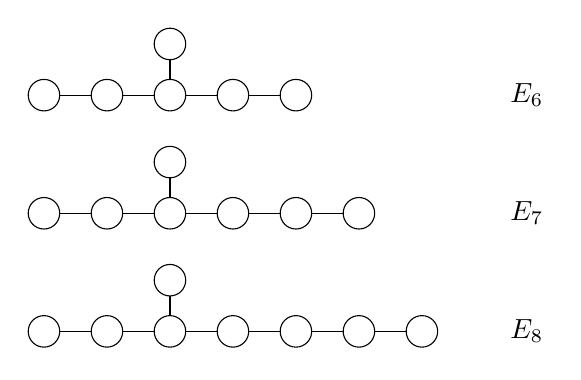
\begin{tikzpicture}[v/.style={circle,draw,inner sep=0pt,minimum size=4mm}]
 \foreach \n/\r/\y in {6/4/0,7/5/-1.5,8/6/-3}
 {
  \foreach \i in {0,...,\r}
    {\node[v] (e\n-\i) at (.8*\i,\y) {};}
  \foreach \i in {1,...,\r}
    {\pgfmathtruncatemacro{\j}{\i-1}\draw (e\n-\j)--(e\n-\i);}
  \node[v] (u\n) at (1.6,\y+.65) {};
  \draw (e\n-2)--(u\n);
  \node[anchor=west] at (5.8,\y) {$E_{\n}$};
 }
\end{tikzpicture}

\small Diagramy $E_6,E_7,E_8$: ramiona mają długości $(1,2,2)$,
$(1,2,3)$ i $(1,2,4)$.
\end{center}

\section{Realizacja i jednoznaczność układów}

\begin{twierdzenie}[Jednoznaczność na podstawie macierzy]
\label{aa:tw:root-uniqueness}
Dwa nierozkładalne skończone układy korzeni z bazami
o tej samej macierzy Cartana są równoważne przez
podobieństwo liniowe przestrzeni euklidesowych.
\end{twierdzenie}
\begin{proof}
Niech $D,D'$ oznaczają diagonalne macierze kwadratów
długości podzielonych przez $2$ w obu bazach.
Na każdej krawędzi iloraz $D_{ii}/D_{jj}$ jest
wyznaczony przez $c_{ji}/c_{ij}$; to samo dla $D'$.
Spójność daje $D'=tD$ dla pewnego $t>0$.
Zatem macierze Grama baz różnią się mnożnikiem $t$.
Liniowe odwzorowanie $L$ przeprowadzające bazę
na bazę spełnia $(Lx,Ly)'=t(x,y)$ dla dowolnych
$x,y$, ponieważ obie strony są dwuliniowe i
zgodne na parach wektorów bazowych.
Z formuły na odbicie wynika
$Ls_{\alpha_i}=s_{L\alpha_i}L$.
Twierdzenie~\ref{aa:tw:weyl-chambers} mówi,
że każdy korzeń jest obrazem korzenia prostego
przez iloczyn odbić prostych; stosując tę równość
dla $L$ i $L^{-1}$ otrzymujemy $L(\Phi)=\Phi'$.
\end{proof}

\begin{twierdzenie}[Realizacja diagramów jednokrawędziowych]
\label{aa:tw:simply-laced-realization}
Niech $C$ będzie jedną z macierzy $A_n,D_n,E_6,E_7,E_8$
z Twierdzenia~\ref{aa:tw:finite-dynkin}. Na $\mathbb R^n$
z bazą standardową $(e_i)$ określmy iloczyn skalarny
$(x,y)=x^{\mathsf T}Cy$ i zbiór
\[
 \Phi_C=\{x\in\mathbb Z^n:x^{\mathsf T}Cx=2\}.
\]
Jest to zredukowany krystalograficzny układ korzeni
z bazą $(e_i)$ i macierzą Cartana $C$.
\end{twierdzenie}
\begin{proof}
Macierz $C$ jest symetryczna i dodatnio określona
na mocy Twierdzenia~\ref{aa:tw:finite-dynkin}.
Istnieje $\delta>0$ takie, że
$x^{\mathsf T}Cx\ge\delta\|x\|_{\mathrm{eukl}}^2$
(dodatnie minimum na sferze jednostkowej).
Zbiór wektorów całkowitych o ograniczonej normie
jest skończony. Każdy $e_i$ należy do $\Phi_C$,
więc korzenie rozpinają przestrzeń.
Wszystkie korzenie mają długość $\sqrt2$,
więc proporcjonalne korzenie różnią się co najwyżej
znakiem. Dla $\alpha,\beta\in\Phi_C$ liczba
$(\alpha,\beta)=\alpha^{\mathsf T}C\beta$ jest całkowita,
a odbicie $s_\alpha(\beta)=\beta-(\alpha,\beta)\alpha$
jest całkowite i zachowuje długość, więc należy
do $\Phi_C$. Ponieważ odbicie jest inwolucją,
przeprowadza zbiór na siebie.

Forma $x^{\mathsf T}Cx$ przyjmuje na $\mathbb Z^n$
wartości parzyste: przekątna jest równa $2$,
a wpisy pozadiagonalne pojawiają się parami.
Dla niezerowego wektora całkowitego jej wartość
jest więc co najmniej $2$.
Jeśli $\beta$ miałby współrzędne obu znaków,
zapiszmy $\beta=u-v$ dla niezerowych wektorów
całkowitych $u,v$ o nieujemnych współrzędnych
i rozłącznych nośnikach. Wtedy
$(u,v)\le0$, bo ich wspólne składniki diagonalne
znikają, a pozostałe wpisy $C$ są niedodatnie.
Stąd $(\beta,\beta)=(u,u)+(v,v)-2(u,v)\ge4$,
sprzecznie z definicją $\Phi_C$.
Współrzędne każdego korzenia mają jeden znak,
więc $(e_i)$ jest bazą układu.
Macierz Cartana tej bazy to $C$, gdyż
$(e_i,e_i)=2$ i $(e_i,e_j)=c_{ij}$.
\end{proof}

\begin{przyklad}[Modele klasyczne]
\label{aa:prz:classical-roots}
W poniższych modelach $e_i$ to standardowe
ortonormalne wektory, a wszystkie wskazane
znaki można wybierać niezależnie.
\[
\begin{array}{c|l|l}
 &\Phi&\text{korzenie proste}\\ \hline
 A_n & e_i-e_j,\ i\ne j,\ 1\le i,j\le n+1
       & e_i-e_{i+1}\ (1\le i\le n)\\
 B_n & \pm e_i,\ \pm e_i\pm e_j,\ i<j
       & e_i-e_{i+1}\ (i<n),\ e_n\\
 C_n & \pm2e_i,\ \pm e_i\pm e_j,\ i<j
       & e_i-e_{i+1}\ (i<n),\ 2e_n\\
 D_n & \pm e_i\pm e_j,\ i<j
       & e_i-e_{i+1}\ (i<n),\ e_{n-1}+e_n
\end{array}
\]
Dla $A_n$ pracujemy w hiperpłaszczyźnie
$\sum x_i=0$ w $\mathbb R^{n+1}$, dla pozostałych
w $\mathbb R^n$; zakresy $n$ są jak w klasyfikacji.

Odbicie względem $e_i-e_j$ zamienia współrzędne
$i,j$, a względem $e_i+e_j$ zamienia je i zmienia
oba znaki. Odbicie względem $e_i$ lub $2e_i$ zmienia
znak jednej współrzędnej. Zatem każdy zbiór jest
zachowany przez wszystkie własne odbicia.
Układy są zredukowane i całkowitość parowań wynika
z podanych długości: korzenie typu $\pm e_i\pm e_j$
mają kwadrat długości $2$ i całkowite iloczyny
skalarne; $\pm e_i$ mają kwadrat długości $1$;
$\pm2e_i$ mają kwadrat długości $4$, lecz ich
iloczyny z każdym korzeniem są parzyste.
Wszystkie podane rodziny korzeni prostych są bazami:
różnice rozpinają hiperpłaszczyznę sumy zerowej,
a w typach $B,C,D$ ostatni wektor ma niezerową
sumę współrzędnych. Dla $i<j$ mamy
$e_i-e_j=\sum_{k=i}^{j-1}(e_k-e_{k+1})$.
W typie $B$ każdy $e_i$ jest nieujemną sumą
korzeni prostych, zatem również $e_i+e_j$.
W typie $C$ piszemy $2e_i=2(e_i-e_n)+2e_n$,
$e_i+e_j=(e_i-e_n)+(e_j-e_n)+2e_n$.
W typie $D$ dla $i<j<n$ piszemy
$e_i+e_j=(e_i-e_{n-1})+(e_j-e_n)+(e_{n-1}+e_n)$,
a dla $j=n$ mamy
$e_i+e_n=(e_i-e_{n-1})+(e_{n-1}+e_n)$.
Wszystkie składniki są nieujemnymi sumami,
pozostałe korzenie są ich przeciwieństwami.
Macierze tych baz mają podane diagramy,
co wynika z iloczynów skalarnych sąsiednich różnic
i ostatniego korzenia.
\end{przyklad}

\begin{przyklad}[Model $F_4$]
\label{aa:prz:f4-roots}
W $\mathbb R^4$ weźmy
\[
 \Phi=\{\pm e_i\}\cup\{\pm e_i\pm e_j:i<j\}
       \cup\left\{\tfrac12(\pm e_1\pm e_2\pm e_3\pm e_4)\right\}.
\]
Zbiór liczy $8+24+16=48$ korzeni i jest zredukowany;
rozpina przestrzeń, ponieważ zawiera $e_i$.
Dla długiego korzenia $\alpha=\pm e_i\pm e_j$
parowanie $2(\beta,\alpha)/(\alpha,\alpha)=(\beta,\alpha)$
jest całkowite nawet dla korzeni połówkowych,
bo dodajemy lub odejmujemy dwie połówki.
Dla krótkiego korzenia $\alpha$ mamy
$(\alpha,\alpha)=1$; iloczyn z korzeniem
połówkowym, jednostkowym lub długim jest
wielokrotnością $1/2$ (dla dwóch połówkowych
suma czterech liczb $\pm1/4$ jest wielokrotnością
$1/2$). Stąd całkowitość.

Odbicia względem korzeni jednostkowych i długich
są zmianami znaków i permutacjami współrzędnych,
więc zachowują $\Phi$. Dla połówkowych wystarczy
sprawdzić $u=(e_1+e_2+e_3+e_4)/2$, ponieważ
zmiany znaków przeprowadzają $u$ na każdy taki
korzeń. Odbicie ma postać $s_u(x)=x-2(x,u)u$.
Dla $x=e_i$ wynikiem jest $e_i-u$, korzeń
połówkowy; przeciwieństwa dają przeciwieństwa.
Dla korzenia długiego iloczyn z $u$ jest $0$ lub
$\pm1$: w pierwszym przypadku korzeń jest ustalony,
w drugim odbicie zastępuje dwie niezerowe współrzędne
dwiema przeciwnymi na dopełniających indeksach.
Dla połówkowego $x$ iloczyn $(x,u)$ jest
$0,\pm1/2,\pm1$. Jeśli wynosi $0$, korzeń jest
ustalony; jeśli $\pm1$, mamy $x=\pm u$, a odbicie
zmienia znak. Jeśli $1/2$, trzy znaki są dodatnie
i jeden ujemny, więc $x-u=-e_i$ dla ujemnego
indeksu. Przypadek $-1/2$ wynika przez zmianę znaku.
To dowodzi zachowania całego zbioru.

Bazę tworzą
$\alpha_1=e_2-e_3$, $\alpha_2=e_3-e_4$,
$\alpha_3=e_4$, $\alpha_4=(e_1-e_2-e_3-e_4)/2$.
Mamy $e_4=\alpha_3$, $e_3=\alpha_2+\alpha_3$,
$e_2=\alpha_1+\alpha_2+\alpha_3$ i
$e_1=2\alpha_4+e_2+e_3+e_4$.
Te równości dowodzą, że wektory tworzą bazę.
Wszystkie $e_i$ i $e_i\pm e_j$ dla $i<j$
mają nieujemne współrzędne w tej bazie:
różnice kolejnych $e_i$ są nieujemnymi sumami,
a sumy również. Korzeń połówkowy o dodatniej
współrzędnej przy $e_1$ ma postać
$\alpha_4+\sum_{i=2}^4\varepsilon_i e_i$,
gdzie $\varepsilon_i$ to $0$ albo $1$.
Pozostałe są przeciwieństwami. Otrzymujemy bazę
układu, z długimi $\alpha_1,\alpha_2$ i krótkimi
$\alpha_3,\alpha_4$, a jedyne niezerowe iloczyny
między różnymi prostymi to
$(\alpha_1,\alpha_2)=-1$, $(\alpha_2,\alpha_3)=-1$,
$(\alpha_3,\alpha_4)=-1/2$. Diagram jest $F_4$.
\end{przyklad}

\begin{przyklad}[Model $G_2$]
\label{aa:prz:g2-roots}
W płaszczyźnie $x_1+x_2+x_3=0$ w $\mathbb R^3$
weźmy sześć krótkich korzeni $e_i-e_j$ ($i\ne j$)
i sześć długich $\pm(2e_i-e_j-e_k)$, gdzie
$\{i,j,k\}=\{1,2,3\}$. Kwadraty długości wynoszą
odpowiednio $2$ i $6$, a zbiór jest zredukowany:
krótkie korzenie mają współrzędną zerową,
długie jej nie mają. Parowania względem krótkich
są całkowite. Dla długiego
$\alpha=2e_i-e_j-e_k$ i dowolnego $\beta$
w tej płaszczyźnie mamy $(\beta,\alpha)=3\beta_i$,
więc parowanie wynosi $\beta_i\in\mathbb Z$.
Odbicia krótkie zamieniają współrzędne,
zaś odbicie długie jest na płaszczyźnie
ujemnością transpozycji współrzędnych $j,k$:
obie izometrie zmieniają znak $\alpha$ i ustalają
prostopadły do niego $e_j-e_k$.
Zatem wszystkie odbicia zachowują zbiór.
Jako bazę bierzemy $\alpha=e_1-e_2$ oraz
$\beta=-2e_1+e_2+e_3$. Są niezależne, a lista
\[
 \alpha,\ \beta,\ \alpha+\beta,\ 2\alpha+\beta,\
 3\alpha+\beta,\ 3\alpha+2\beta
\]
ma w standardowych współrzędnych postać
\[
 (1,-1,0),\ (-2,1,1),\ (-1,0,1),\
 (0,-1,1),\ (1,-2,1),\ (-1,-1,2).
\]
Są to sześć różnych korzeni, żadne dwa nie są
przeciwieństwami, a ich współrzędne względem
$(\alpha,\beta)$ są nieujemne. Razem z przeciwieństwami
wyczerpują wszystkie dwanaście korzeni.
Iloczyn $(\alpha,\beta)=-3$, więc macierz bazy
to $\begin{pmatrix}2&-3\\-1&2\end{pmatrix}$.
\end{przyklad}

\begin{wniosek}[Klasyfikacja układów korzeni]
\label{aa:cor:root-classification}
Każdy nierozkładalny zredukowany krystalograficzny
skończony układ korzeni jest, z dokładnością do
podobieństwa przestrzeni euklidesowych, jednym
z typów $A_n,B_n,C_n,D_n,E_6,E_7,E_8,F_4,G_2$,
z zakresami jak w Twierdzeniu~\ref{aa:tw:finite-dynkin}.
\end{wniosek}
\begin{proof}
Istnienie bazy i macierzy typu skończonego wynika
z Twierdzeń~\ref{aa:tw:root-base}
i~\ref{aa:tw:root-cartan}. Klasyfikujemy tę macierz
przez Twierdzenie~\ref{aa:tw:finite-dynkin}.
Realizacje jednokrawędziowe daje
Twierdzenie~\ref{aa:tw:simply-laced-realization},
a pozostałe podane modele $B,C,F_4,G_2$.
Spójność każdej otrzymanej macierzy daje
nierozkładalność realizacji. Jednoznaczność dla
ustalonej macierzy daje Twierdzenie~\ref{aa:tw:root-uniqueness}.
Jeśli podobieństwo przeprowadza jeden układ na drugi,
przeprowadza także jego bazę na pewną bazę drugiego
układu i zachowuje wszystkie parowania Cartana,
ponieważ iloczyny skalarne i kwadraty długości
zmieniają się o ten sam dodatni czynnik.
Na mocy Twierdzenia~\ref{aa:tw:weyl-chambers}
wszystkie bazy drugiego układu są równoważne przez
izometrię z jego grupy Weyla. Macierze różnią się
więc tylko jednoczesną permutacją indeksów.
Różne diagramy z listy (po utożsamieniu $B_2$ i $C_2$)
nie mogą zatem opisywać podobnych układów.
\end{proof}

\section{Przykład grupy Weyla i powrót do grafów McKaya}

\begin{przyklad}[Grupy Weyla typów klasycznych]
Dla modelu $A_n$ z Przykładu~\ref{aa:prz:classical-roots}
odbicia są transpozycjami współrzędnych, które
generują $S_{n+1}$. Działanie na hiperpłaszczyźnie
jest wierne, ponieważ permutacja ustalająca wszystkie
różnice $e_i-e_j$ musi ustalać każdą uporządkowaną
parę różnych indeksów. Stąd $W(A_n)\simeq S_{n+1}$.
Dla $B_n,C_n$ odbicia generują wszystkie permutacje
i wszystkie niezależne zmiany znaków współrzędnych.
Każde takie przekształcenie ma jednoznaczny rozkład
na zmianę znaków i permutację, więc grupa jest
iloczynem półprostym $(C_2)^n\rtimes S_n$
o rzędzie $2^n n!$.
Dla $D_n$ odbicia zachowują parzystość liczby zmienionych
znaków. Wszystkie permutacje są generowane przez
odbicia względem różnic, a zmiana znaków dokładnie
dwóch współrzędnych jest iloczynem odbić względem
$e_i-e_j$ i $e_i+e_j$. Każdą parzystą rodzinę
zmian znaków rozkładamy na takie pary.
Zatem $W(D_n)$ jest iloczynem półprostym podgrupy
parzystych zmian znaków $(C_2)^{n-1}$ i $S_n$,
o rzędzie $2^{n-1}n!$.
\end{przyklad}

\begin{wniosek}[Od diagramu afinicznego do zwykłego]
\label{aa:cor:mckay-finite-dynkin}
Niech $G$ będzie nietrywialną skończoną podgrupą
$\operatorname{SL}_2(\mathbb C)$, a $A$ jej macierzą
McKaya. Macierz uzyskana z $2I-A$ przez usunięcie
wiersza i kolumny reprezentacji trywialnej ma typ
$A_{m-1}$ dla $C_m$, $D_{n+2}$ dla $\operatorname{Dic}_n$
oraz odpowiednio $E_6,E_7,E_8$ dla $2T,2O,2I$.
\end{wniosek}
\begin{proof}
Dodatnia określoność wynika ze
Stwierdzenia~\ref{aa:prop:mckay-cartan}.
Dla cyklu $\widetilde A_{m-1}$ usunięcie wierzchołka
daje ścieżkę $m-1$ wierzchołków; dla $m=2$
pozostaje macierz $(2)$ typu $A_1$.
Dla $\widetilde D_4$ usunięcie liścia daje trzy
ramiona długości $1$. Dla $\widetilde D_{n+2}$
z $n\ge3$ trywialny wierzchołek jest liściem
przy końcu ścieżki: po jego usunięciu drugi koniec
jest jedynym rozgałęzieniem, z ramionami
$(1,1,n-1)$, co daje $D_{n+2}$.
Dla $\widetilde E_6,\widetilde E_7,\widetilde E_8$
liść o wymiarze jeden znajduje się na ramieniu
długości odpowiednio $2,3,5$. Skrócenie jednego
takiego ramienia daje $(1,2,2),(1,2,3),(1,2,4)$.
To są dokładnie diagramy zwykłe z
Twierdzenia~\ref{aa:tw:finite-dynkin}.
\end{proof}

Związek jest algebraiczno-kombinatoryczny. Konstrukcja
algebr Liego z układów korzeni, pełna teoria afinicznych
macierzy Cartana i geometryczna odpowiedniość McKaya
wymagają dalszych rozdziałów; nie zakładaliśmy ich
w powyższych dowodach.
